\section{Atividade 3}

\subsection{Descrição do Modelo e Análise de Sistema}
Nesta atividade, desenvolvemos e analisamos a função de transferência de um sistema massa-mola-amortecedor, utilizando os seguintes parâmetros específicos, essenciais para entender a dinâmica do sistema:
\begin{itemize}
    \item Massa (\( m \)): 10 kg, que influi diretamente na inércia do sistema, afetando como o sistema responde a forças externas.
    \item Coeficiente de amortecimento (\( C \)): 7 Ns/m, crucial para atenuar as oscilações e determinar a rapidez com que o sistema atinge um estado de equilíbrio.
    \item Constante da mola (\( K \)): 5 N/m, que define a rigidez do sistema e afeta a frequência das oscilações naturais.
\end{itemize}
A função de transferência modelada é expressa por:
\[
    G(s) = \frac{1}{10s^2 + 7s + 5}
\]

\subsection{Código Scilab para a função de transferência em malha fechada}
\begin{lstlisting}[language=Scilab, caption=Código Scilab para a função de transferência em malha fechada]
    // Parametros do sistema
    m = 10;  // massa
    c = 7;   // coeficiente de amortecimento
    k = 5;   // constante da mola

    // Definindo a funcao de transferencia
    s = %s; // Variavel complexa s
    G = syslin('c', 1 / (m*s^2 + C*s + K));

    // Calculando os polos e exibindo
    polos = roots(G.den);
    disp("Polos da funcao de transferencia:");
    disp(polos);

    // Parametros do sistema de segunda ordem
    wn = sqrt(K / m);
    zeta = C / (2 * sqrt(m * K));
    Kp = 1 / K;  // Ganho estatico para a entrada degrau
    disp("Frequencia natural nao-amortecida (wn): " + string(wn));
    disp("Coeficiente de amortecimento (zeta): " + string(zeta));
    disp("Ganho estatico (Kp): " + string(Kp));

    // Plotando a resposta ao impulso do sistema
    t = 0:0.01:10;
    y = csim('imp', t, G);
    plot(t, y);
    xlabel("Tempo (s)");
    ylabel("Resposta ao impulso");
    title("Resposta ao impulso do sistema massa-mola-amortecedor");
\end{lstlisting}


\subsection{Cálculo dos Polos e Parâmetros do Sistema}
Os polos da função de transferência são essenciais para entender como o sistema responde a estímulos externos:
\begin{itemize}
    \item Polo 1: \( -0.35 + 0.614j \)
    \item Polo 2: \( -0.35 - 0.614j \)
\end{itemize}
Estes polos indicam uma resposta oscilatória amortecida, característica de um sistema subamortecido devido à sua parte real negativa e parte imaginária não nula.

Os parâmetros do sistema de segunda ordem são determinados como segue:
\begin{itemize}
    \item Frequência natural não-amortecida (\( \omega_n \)): 0.707 rad/s, que descreve a frequência natural de oscilação do sistema na ausência de amortecimento.
    \item Coeficiente de amortecimento (\( \zeta \)): 0.495, refletindo a eficácia do amortecimento em reduzir as oscilações.
    \item Ganho estático (\( K_p \)): 0.2, representando a resposta do sistema em estado estacionário a uma entrada de degrau unitário.
\end{itemize}

\subsection{Resposta ao Impulso}
Utilizando o software Scilab, simulamos a resposta ao impulso do sistema, como ilustrado abaixo. A resposta apresenta um pico inicial significativo seguido por um decaimento exponencial das oscilações, um comportamento típico de sistemas subamortecidos.
\begin{figure}[H]
    \centering
    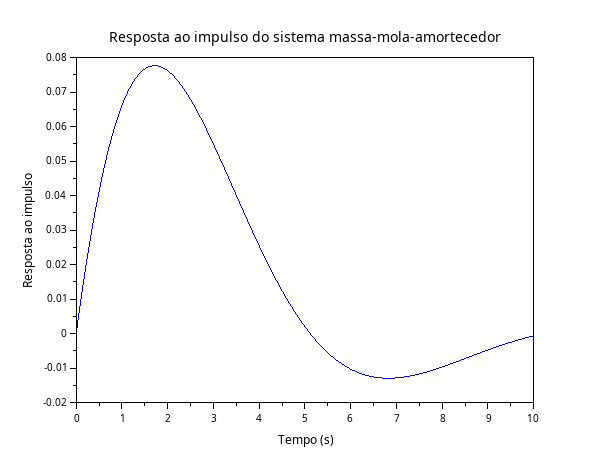
\includegraphics[width=0.8\textwidth]{atividades/3-atividade/assets/resposta-ao-impulso.png}
    \caption{Resposta ao impulso do sistema massa-mola-amortecedor}
\end{figure}

\subsection{Discussão}
A análise dos polos e dos parâmetros do sistema demonstra que ele é bem projetado para equilibrar uma resposta rápida com oscilações controladas, minimizando as oscilações excessivas sem comprometer a agilidade da resposta. Esta característica é crucial para sistemas de controle que exigem precisão e estabilidade.

\subsection{Conclusões}
Esta atividade ofereceu uma visão profunda sobre como os parâmetros físicos — massa, amortecimento e rigidez — influenciam a resposta dinâmica de um sistema. Estes insights são fundamentais para o design e a análise de sistemas de controle adequados, que são essenciais em aplicações práticas onde a precisão e estabilidade são críticas.
